\documentclass[12pt]{report}			% Začátek dokumentu
\usepackage{MP}				
\usepackage{amsmath}
\usepackage{mathtools}
\usepackage{graphicx}		% Import stylu
\usepackage{indentfirst}
\author{David Kolář}
\title{Geometrická posloupnost a posloupnosti z ní odvozené}
\date{14. února 2023}
\vedouci{Mgr. Michaela Petrová}
\place{V Českých Budějovicích}
\skolnirok{2022/2023}
\logo{
\includegraphics[scale=1.25]{GJ8_logotyp}}

\begin{document}
\pagenumbering{roman}                   % číslování stránek římskými číslicemi
	\mytitlepage						% Vygenerování titulní strany
	
	\prohlaseni{
		Prohlašuji, že tato maturitní práce je mým původním autorským dílem, které jsem vypracoval samostatně. Všechny zdroje, prameny a literaturu, které jsem při vypracování
používal nebo z nich čerpal, v práci řádně cituji s uvedením úplného odkazu na příslušný
zdroj.

	}	
	
	\abstrakt{
	
				% Abstrakt
	}{
							% Klíčová slova
	}
	
	\podekovani{
Rád bych vyjádřil hlubokou vděčnost vedoucí mojí práce, paní Michaele Petrové, za její neocenitelné vedení, mnoho užitečných rad a hlavně za její trpělivost. 
Dále bych rád poděkoval svému dobrému příteli Lukáši Knotovi, velkému zdroji inspirace, za poskytnutí nového pohledu na mou práci, konstruktivní kritiku a zpětnou vazbu.				% Poděkování
	}
	
   {\tableofcontents\newpage}			% Obsah
	
\addtocounter{page}{1}		% Posunutí countru stránek
\pagenumbering{arabic}		% Číslování stránke arabskými číslicemi
	\chapter*{Úvod}
Vždy mě fascinovaly matematické posloupnosti a jejich součty, a proto jsem se rozhodl na toto téma zpracovat svou maturitní práci. V matematice a informatice se při určování časové a prostorové složitosti algoritmu často spoléháme na vyhodnocení právě součtu členů posloupností. Proto může být nalezení uzavřeného tvaru, neboli součtového vzorce posloupnosti, nesmírně užitečné.

Moje maturitní práce je rozdělena na dvě části: teoretickou část a praktickou část. 
V teoretické části začnu definicí toho, co je to matematická posloupnost a pojednám o jejích různých typech a vlastnostech. Poté se budu věnovat specifickým vlastnostem geometrické a aritmetické posloupnosti, včetně jejich součtových vzorců, a ukážu uplatnění geometrické posloupnosti při určování časové a prostorové složitosti. Dále představím pojem aritmeticko-geometrické posloupnosti a vysvětlím, čím se liší od ostatních typů posloupností. Nakonec ukážu svou vlastní posloupnost, kterou jsem objevil při studiu.

V praktické části své práce uvedu důkaz součtu geometrické, aritmeticko-geometrické a mojí posloupnosti. 

Celkově si má maturitní práce klade za cíl poskytnout základní přehled týkající se matematických posloupností, konkrétně geometrické, aritmeticko-geometrické a mojí posloupnosti a představit mé poznatky a myšlenky na toto téma.

	
	
	\part{Teoretická část}
	
		\chapter{Zavedení pojmu posloupnost}
		
			
			\section{Definice a vysvětlení pojmu funkce}
Pro zavedené pojmu posloupnost je nutné nejprve zavést a vysvětlit obecnější pojem funkce. V matematice označuje pojem funkce vztah mezi množinou vstupů a množinou výstupů s vlastností, že každému vstupu je přiřazen právě s jeden výstup. Vstup funkce se nazývá argument a výstup se nazývá hodnota funkce.

Funkce jsou důležitým nástrojem v matematice a používají se v mnoha různých oblastech, včetně fyziky, inženýrství, ekonomie a dalších. Lze je analyzovat pomocí různých matematických technik jako je infinitezimální počet a algebra. Nejprve zavedeme základní pojmy týkající se funkcí.


				\subsection{Formální definice}
Definice 1 [funkce]: Funkce na množině $\mathbb{D} \subset \mathbb{R}$ je předpis, který každému číslu z množiny  $\mathbb{D}$ přiřazuje právě jedno reálné číslo.

				\subsection{Definiční obor}
Pokud máme funkci $f$, pak množině $D$, na které je funkce $f$ definována, se říká \emph{definiční obor} funkce $f$ a značí se $D(f)$.
				\subsection{Obor hodnot}
Obor hodnot je množina všech reálných čísel $y$, která lze dostat jako výstupní hodnotu funkce $f$, jestliže se za $x$ dosadí všechny přípustné hodnoty z $D(f)$. Obor hodnot funkce $f$ se značí $H(f)$.
				\subsection{Zadání funkce}
Funkci lze zadat několika způsoby, ty nejvýznamnější si ukážeme na funkci $\sin(x)$.

					\subsubsection{Předpisem}
					\begin{itemize}
					\item $f:\quad y = \sin(x)$
					\item $y = \sin(x)$
					\item $x \to \sin(x)$
					\end{itemize}
Toto vše jsou validní notace předpisu funkce. Při používání předpisu je nezbytné určit definiční obor.
				\subsubsection{Tabulkou}
První řádek představuje vstup funkce $x$ a druhý řádek výstup funkce $sin(x)$.
\begin{center}
\begin{tabular}{ | m{1cm} | m{1cm}| m{1cm} | m{1cm} |m{1cm} |m{1cm} |} 
\hline
  $x$ & $0$ & $\frac{\pi}{6}$ & $\frac{\pi}{4}$ & $\frac{\pi}{3}$ & $\frac{\pi}{2}$ \\
\hline
	$\sin(x)$ & $0$ & $\frac{1}{2}$ & $\frac{\sqrt{2}}{2}$ & $\frac{\sqrt{3}}{2}$ & $1$ \\
\hline
\end{tabular}
\end{center}
				\subsubsection{Grafem}
Graf funkce $\sin(x)$ s oborem definice $D(f) = \langle 0, 2\pi \rangle$. Pro vizualizaci jsem použil program Geogebra.
\begin{center}
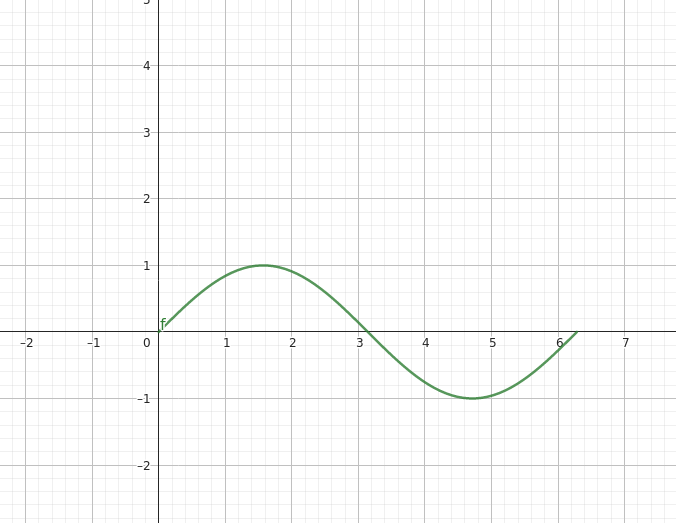
\includegraphics[scale=0.4]{./images/graf.png}
\end{center}
		\section{Vysvětlení pojmu posloupnost}
Posloupnost je funkce definovaná na množině přirozených čísel, což jsou celá kladná čísla (1, 2, 3 atd.). Stejně jako u funkce tedy platí, že se jedná o vztah mezi množinou vstupů a množinou možných výstupů s vlastností, že ke každému vstupu je přiřazený právě jeden výstup. Definiční obor posloupnosti může být buď konečná množina, pak se posloupnost nazývá \emph{konečná}, nebo \emph{nekonečná} množina, pak se posloupnost nazývá \emph{nekonečná}.
		\section{Značení}
Prvky z definičního oboru posloupnosti $(a_n)$ budu označovat $n$ a funkční hodnoty posloupnosti $(a_n)$ označovat $a_n$. Platí tedy, že $n$-tému prvku je přiřazena hodnota $a_n$.
		\subsection{Značení nekonečné posloupnosti}
Nekonečné posloupnosti budu značit $(a_n)_{n=1}^{\infty} $.
		\subsection{Značení konečné posloupnosti}
Konečné posloupnosti budu značit jako $(a_n)_{n=1}^k$ kde přirozené číslo $k$ označuje maximální velikost $n$. Definiční obor posloupnosti $(a_n)$ tedy zahrnuje všechna přirozená čísla od $1$ do $k$. 

Zápisem ve tvaru $n \in \{1, \dots, k\}$ vyjadřuji, že $n$ nabývá hodnotu všech přirozených čísel od $1$ do $k$.

\section{Zadání posloupnosti}
Posloupnost lze zadat různými způsoby v závislosti na povaze posloupnosti, potřebách dané situace a preferencích osoby, která je používá.

Jedním ze způsobů vyjádření posloupnosti je rekurentní vzorec, který definuje každý člen posloupnosti pomocí jeho předchozích členů. 

Dalším způsobem vyjádření posloupnosti je pomocí vzorce, který definuje n-tý člen posloupnosti an pomocí proměnné n. Tento způsob může být užitečný třeba pro posloupnosti, které mají jednoduchý vzorec a lze je snadno definovat. To platí například pro aritmetickou nebo geometrickou posloupnost. 
Posloupnost lze také vyjádřit výčtem hodnot a to buď graficky, nebo pomocí tabulky.  


	\part{Praktická část}

\section{Výpisy použitých programů}

\lipsum[1]	

Výpis programu \nameref{lst:hello_world}  naleznete ve výpise \ref{lst:hello_world}.

\begin{lstlisting}[title={Program hello.c}, caption={hello.c}, label={lst:hello_world}]
#include <stdio.h>
#define CISLO 10

int main(void) {
	int i = CISLO;

	print("Hello World!\n");
	print("%d", i);

	return (0);
}
\end{lstlisting}

\lipsum[1]	

\begin{lstlisting}[numbers=none, title={Příklad výstupního souboru}]
11.0524
5.5954
6.7996
13.8584
15.1357
Soucet: 52.4415
\end{lstlisting}

	\chapter*{Závěr}
	
		\lipsum[1]
	
	\nocite{*}
    \printbibliography					% Vytvoří seznam literatury
	\addcontentsline{toc}{chapter}{Bibliografie}
    \printglossary[title={Zkratky}]		% Vytvoří seznam zkratek
    \listoffigures						% Vytvoří seznam obrázků
    \listoftables						% Vytvoří seznam tabulek

    \begin{appendices}
	\chapter{Fotky z pokusů}	
	\lipsum[1]
    	%\pitem{Fotky z pokusů}
    	%\eitem{Vlastní program}
    	%\eitem{Dokumentace}
    	%\eitem{Testovací data}
	\chapter{Příloha další }
	\end{appendices}
\end{document}
